\chapter{Nonlinear systems}

Consider a 2-dimensional nonlinear system:
\begin{equation*}
\begin{cases}
\dot{x} = f(x, y) \\
\dot{y} = g(x, y)
\end{cases}
\end{equation*}

We cannot isolate an $A$ from this system and so our previous method of finding a solution doesn't work. However, we can characterize the behaviour of the system.

Suppose $
\begin{bmatrix}
x^{*} \\
y^{*}
\end{bmatrix}
$
is a fixed point of the system, that is:
\begin{equation*}
\begin{cases}
f(x^{*}, y^{*}) = 0 \\
g(x^{*}, y^{*}) = 0
\end{cases}
\end{equation*}

We have specifically chosen fixed points where the system is at rest (i.e. no change).

We consider a small perturbation around the fixed point:
\begin{align*}
u = x - x^{*} \quad &\text{and} x = x^{*} + u \\ 
v = y - y^{*} \quad &\text{and} y = y^{*} + v
\end{align*}
such that $u$ and $v$ are small.

Then, apply $\dot{u}$:
\begin{align*}
\dot{u} = \dot{x} &= f(x, y) \\
&= f(x^{*} + u, y^{*} + v) \\
&\text{ applying Taylor expansion around the fixed point } (x^{*}, y^{*}) \\
&= f(x^{*}, y^{*}) + u \frac{\partial f}{\partial x} (x^{*}, y^{*}) + v \frac{\partial f}{\partial y} (x^{*}, y^{*}) + \cdots \\
&= 0 + u \frac{\partial f}{\partial x} (x^{*}, y^{*}) + v \frac{\partial f}{\partial y} (x^{*}, y^{*}) + \cdots
\end{align*}

A similar process can be applied to $\dot{v}$:
\begin{align*}
\dot{v} = \dot{y} &= g(x, y) \\
&= g(x^{*} + u, y^{*} + v) \\
&\text{ applying Taylor expansion around the fixed point } (x^{*}, y^{*}) \\
&= g(x^{*}, y^{*}) + u \frac{\partial g}{\partial x} (x^{*}, y^{*}) + v \frac{\partial g}{\partial y} (x^{*}, y^{*}) + \cdots \\
&= 0 + u \frac{\partial g}{\partial x} (x^{*}, y^{*}) + v \frac{\partial g}{\partial y} (x^{*}, y^{*}) + \cdots
\end{align*}

The higher order terms are negligible because $u$ and $v$ (which are $\delta x$ and $\delta y$) are small. So we can approximate the system as:
\begin{equation*}
\begin{cases}
\dot{u} = u \frac{\partial f}{\partial x} (x^{*}, y^{*}) + v \frac{\partial f}{\partial y} (x^{*}, y^{*}) \\
\dot{v} = u \frac{\partial g}{\partial x} (x^{*}, y^{*}) + v \frac{\partial g}{\partial y} (x^{*}, y^{*})
\end{cases}
\end{equation*}

Essentially, around the fixed point, the system behaves like a linear system. We can analyze the stability of the fixed point by analyzing the eigenvalues of the Jacobian matrix at that point.

Then, writing the system in matrix form:
\begin{equation*}
\begin{bmatrix}
\dot{u} \\
\dot{v}
\end{bmatrix}
=
\begin{bmatrix}
\frac{\partial f}{\partial x} (x^{*}, y^{*}) & \frac{\partial f}{\partial y} (x^{*}, y^{*}) \\
\frac{\partial g}{\partial x} (x^{*}, y^{*})
& \frac{\partial g}{\partial y} (x^{*}, y^{*})
\end{bmatrix}
\begin{bmatrix}
u \\
v
\end{bmatrix}
\end{equation*}

\dfn{Jacobian matrix}{
The Jacobian matrix of a system of nonlinear equations is the matrix of all first-order partial derivatives of the system. In this case, the Jacobian matrix is:
\begin{equation*}
J =
\begin{bmatrix}
f_x (x^{*}, y^{*}) & f_y (x^{*}, y^{*}) \\
g_x (x^{*}, y^{*}) & g_y (x^{*}, y^{*})
\end{bmatrix}
\end{equation*}
}

Near $(x^{*}, y^{*})$, the system behaves like a linear system with matrix $J$, provided $J$ is not degenerate (i.e. has non-zero eigenvalues). 

\ex{Example}{
    Consider the system:
    \begin{equation*}
        \dot{x} = -x + x^3 \\
        \dot{y} = -y
    \end{equation*}
    This system is convenient because of the decoupled $x$ and $y$ components.

    We start by finding the fixed points:
    \begin{align*}
    0 &= -x + x^3 \\
    &= x(x^2 - 1) \\
    \implies x &= 0, 1, -1  
    \end{align*}
    Then, finding the corresponding $y$ values:
    \begin{align*}
    0 &= -y \\
    \implies y &= 0
    \end{align*}
    So the fixed points are $(0, 0), (1, 0), (-1, 0)$.

    To compute the nullclines, we set $\dot{x} = 0$ and $\dot{y} = 0$:
    \begin{align*}
    x\text{-nullcline: } 0 &= -x + x^3 \\
    &= x(x^2 - 1) \\
    \implies x &= 0, 1, -1 \\
    y\text{-nullcline: } 0 &= -y \\
    \implies y &= 0
    \end{align*}

    Next, we compute the Jacobian matrix at each fixed point:
    \begin{align*}
    J(x, y) &=
    \begin{bmatrix}
    -1 + 3x^2 & 0 \\
    0 & -2
    \end{bmatrix} \\
    J(0, 0) &=
    \begin{bmatrix}
    -1 & 0 \\
    0 & -2
    \end{bmatrix} \\
    J(\pm 1, 0) &=
    \begin{bmatrix}
    2 & 0 \\
    0 & -2
    \end{bmatrix}
    \end{align*}

    The eigenvalues of $J(0, 0)$ are $-1$ and $-2$, which are both negative, so $(0, 0)$ is a stable fixed point. The eigenvalues of $J(\pm 1, 0)$ are $2$ and $-2$, which have opposite signs, so $(\pm 1, 0)$ are saddle points.
}

\begin{mdframed}
\subsection{Sketching phase portraits for nonlinear systems}
To sketch the phase portrait for a nonlinear system, we can follow these steps:
\begin{enumerate}
    \item Find the fixed points of the system by solving $f(x, y) = 0$ and $g(x, y) = 0$. The intersection of the nullclines will give us the fixed points.
    \item Find the nullclines of the system by solving $f(x, y) = 0$ and $g(x, y) = 0$ separately. The nullclines will help us determine the direction of the flow in different regions of the phase plane.
    \item For each nullcline, pick a test point in each region defined by the nullclines and determine the direction of the flow at that point. For example, for the $x$-nullcline(s), test different values of $y$ to determine whether $\dot{x}$ is positive or negative in each region. Similarly, for the $y$-nullcline(s), test different values of $x$ to determine whether $\dot{y}$ is positive or negative in each region.
    \item Sketch the nullclines. Then, along each nullcline, draw arrows indicating the direction of the flow (positive or negative) based on the regions found by the test points.
    \item Extend the flow lines at the nullclines.
\end{enumerate}
\begin{center}
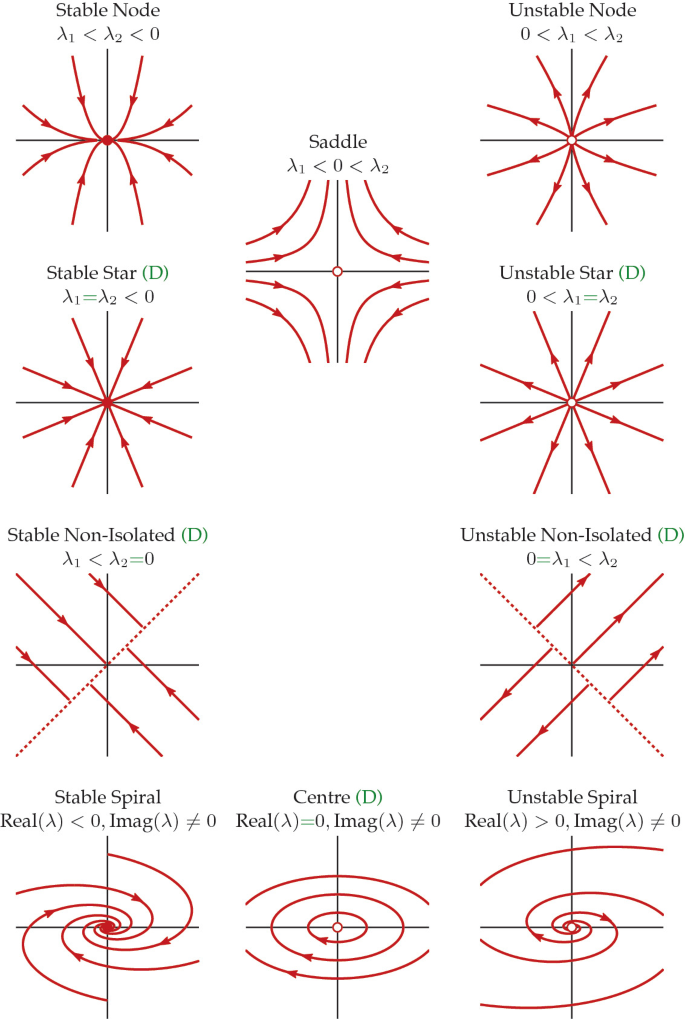
\includegraphics[width=0.9\textwidth]{images/nonlinear_systems/fixed_points.png}
\end{center}
\end{mdframed}

